%version 1.00,	date 12/05/2016	auteur(s) Pierre Porche
\speaker{\Juliana}

\begin{frame}
\frametitle{Développement frontend}
\begin{block}{Technologies utilisées}
	\begin{itemize}
		\item TWIG
		\item CSS
		\item Bootstrap
		\item jQuery
	\end{itemize}
\end{block}
\end{frame}

\begin{frame}
\frametitle{Développement frontend}



      \begin{figure}[r]
		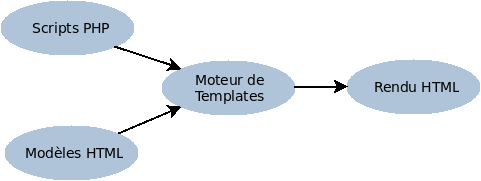
\includegraphics[scale=0.3]{images/moteursTemp.png}
		\caption{Moteurs de templates}
	  \end{figure}
\begin{block}{TWIG: Le moteur de templates }
	
		\begin{itemize}
			\item Séparation du code HTML du code PHP
			\item Héritage de templates
			\item Intégré directement dans le framework Symfony3
		\end{itemize}
\end{block}
\end{frame}

\begin{frame}
\frametitle{Développement frontend}
\begin{block}{ CSS et Bootstrap }
	\begin{itemize}
		\item Génération de vues responsives
		\item Grande collection de composants
		\item Communauté qui propose des centaines d'autres composants
	\end{itemize}
\end{block}
\end{frame}

\begin{frame}
\frametitle{Développement frontend}
\begin{block}{jQuery }
	\begin{itemize}
		\item Dynamisme côté client
		\item Modification de la structure HTML et aussi des styles
		\item Documentation riche et complète
	\end{itemize}
\end{block}
\end{frame}

\begin{frame}
\frametitle{Responsive design}
	\begin{multicols}{2}
		\begin{figure}[!h]
			\begin{center}
				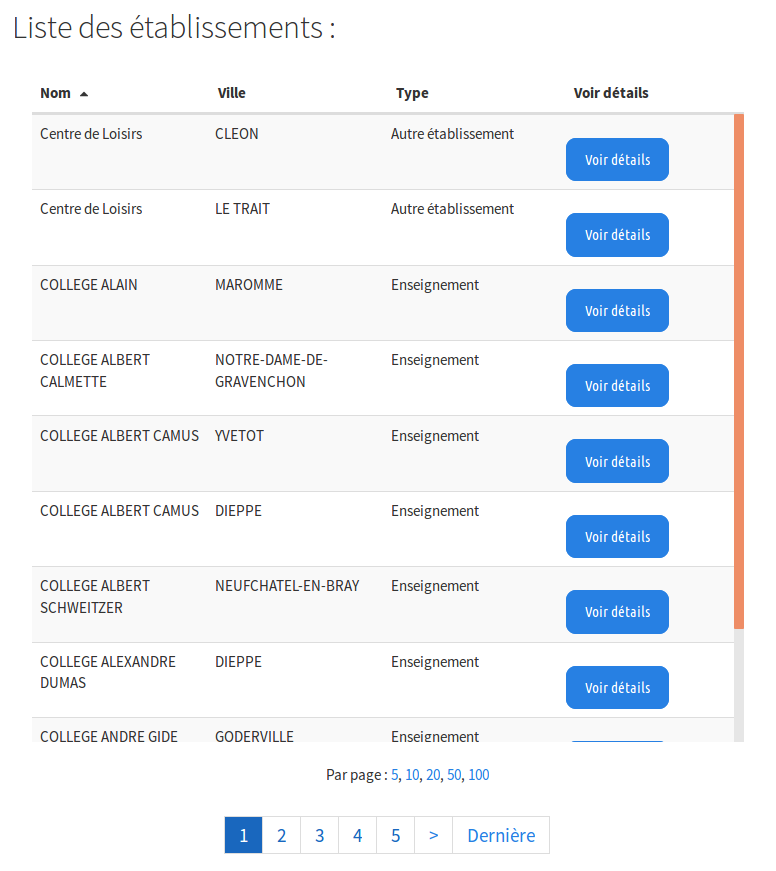
\includegraphics[scale=0.19]{images/screenshot1.png}

				\caption{Listes grand écran }
			\end{center}
		\end{figure}
		\begin{figure}[!h]
			\begin{center}
				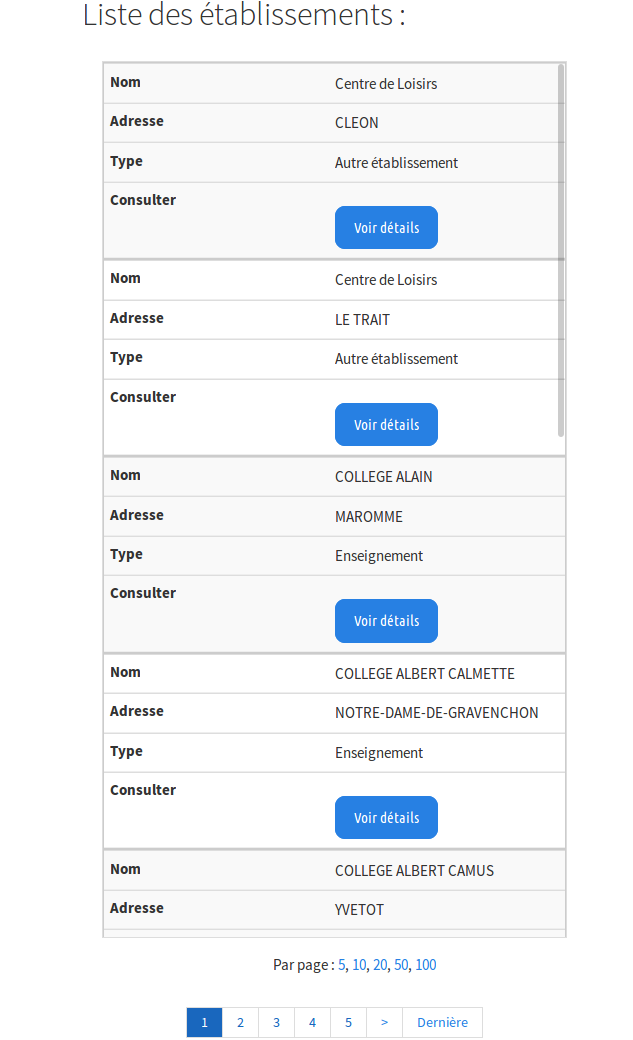
\includegraphics[scale=0.16]{images/screenshot2.png}
				\caption{Listes petit écran }
			\end{center}
		\end{figure}
	\end{multicols}

\end{frame}

